%%%%%%%%%%%%%%%%%%%%%%%%%%%%%%%%%%%%%%%%%%%%%%%%%%%%%%%%%%%%%%%%%%%%%%%%%%%%%%%
%                       CARREGA DE LA CLASSE DE DOCUMENT                      %
%                                                                             %
% Les opcions admissibles son:                                                %
%      12pt / 11pt            (cos dels tipus de lletra; no feu servir 10pt)  %
%                                                                             %
% catalan/spanish/english     (llengua principal del treball)                 %
%                                                                             % 
% french/italian/german...    (si necessiteu fer servir alguna altra llengua) %
%                                                                             %
% listoffigures               (El document inclou un Index de figures)        %
% listoftables                (El document inclou un Index de taules)         %
% listofquadres               (El document inclou un Index de quadres)        %
% listofalgorithms            (El document inclou un Index d'algorismes)      %
%                                                                             %
%%%%%%%%%%%%%%%%%%%%%%%%%%%%%%%%%%%%%%%%%%%%%%%%%%%%%%%%%%%%%%%%%%%%%%%%%%%%%%%
\PassOptionsToPackage{table}{xcolor}

\documentclass[11pt,catalan,listoffigures,listoftables]{tfgetsinf}
\renewcommand{\labelitemii}{$\diamond$}

\setlength{\arrayrulewidth}{1mm}
\setlength{\tabcolsep}{10pt}
\renewcommand{\arraystretch}{1.3}
 
\newcolumntype{s}{>{\columncolor[HTML]{AAACED}} p{3cm}}
 
\arrayrulecolor[HTML]{000000}

%%%%%%%%%%%%%%%%%%%%%%%%%%%%%%%%%%%%%%%%%%%%%%%%%%%%%%%%%%%%%%%%%%%%%%%%%%%%%%%
%                     CODIFICACIO DEL FITXER FONT                             %
%                                                                             %
%    windows fa servir normalment 'ansinew'                                   %
%    amb linux es possible que siga 'latin1' o 'latin9'                       %
%    Pero el mes recomanable es fer servir utf8 (unicode 8)                   %
%                                          (si el vostre editor ho permet)    % 
%%%%%%%%%%%%%%%%%%%%%%%%%%%%%%%%%%%%%%%%%%%%%%%%%%%%%%%%%%%%%%%%%%%%%%%%%%%%%%%
\usepackage{hyperref}
\usepackage{float}
\usepackage{lmodern,textcomp}
\usepackage[utf8]{inputenc} 
\definecolor{forestgreen}{RGB}{34,139,34}
\definecolor{costumyellow}{RGB}{255,185,1}

%%%%%%%%%%%%%%%%%%%%%%%%%%%%%%%%%%%%%%%%%%%%%%%%%%%%%%%%%%%%%%%%%%%%%%%%%%%%%%%
%                        ALTRES PAQUETS I DEFINICIONS                         %
%                                                                             %
% Carregueu aci els paquets que necessiteu i declareu les comandes i entorns  %
%                                          (aquesta seccio pot ser buida)     %
%%%%%%%%%%%%%%%%%%%%%%%%%%%%%%%%%%%%%%%%%%%%%%%%%%%%%%%%%%%%%%%%%%%%%%%%%%%%%%%



%%%%%%%%%%%%%%%%%%%%%%%%%%%%%%%%%%%%%%%%%%%%%%%%%%%%%%%%%%%%%%%%%%%%%%%%%%%%%%%
%                        DADES DEL TREBALL                                    %
%                                                                             %
% titol, alumne, tutor i curs academic                                        %
%%%%%%%%%%%%%%%%%%%%%%%%%%%%%%%%%%%%%%%%%%%%%%%%%%%%%%%%%%%%%%%%%%%%%%%%%%%%%%%

\title{Implementació de xarxa social per a persones amb diversitat funcional}
\author{David Aleu Moseguí}
\tutor{Xavier Burgués Illa}
\curs{2016-2017}

%%%%%%%%%%%%%%%%%%%%%%%%%%%%%%%%%%%%%%%%%%%%%%%%%%%%%%%%%%%%%%%%%%%%%%%%%%%%%%%
%                     PARAULES CLAU/PALABRAS CLAVE/KEY WORDS                  %
%                                                                             %
% Independentment de la llengua del treball, s'hi han d'incloure              %
% les paraules clau i el resum en els tres idiomes                            %
%%%%%%%%%%%%%%%%%%%%%%%%%%%%%%%%%%%%%%%%%%%%%%%%%%%%%%%%%%%%%%%%%%%%%%%%%%%%%%%

\keywords{????, ?????????, ????, ?????????????????} % Paraules clau 
         {?????, ???, ???????????????}              % Palabras clave
         {?????, ????? ?????, ?????????????}        % Key words

%%%%%%%%%%%%%%%%%%%%%%%%%%%%%%%%%%%%%%%%%%%%%%%%%%%%%%%%%%%%%%%%%%%%%%%%%%%%%%%
%                              INICI DEL DOCUMENT                             %
%%%%%%%%%%%%%%%%%%%%%%%%%%%%%%%%%%%%%%%%%%%%%%%%%%%%%%%%%%%%%%%%%%%%%%%%%%%%%%%

\begin{document}

%%%%%%%%%%%%%%%%%%%%%%%%%%%%%%%%%%%%%%%%%%%%%%%%%%%%%%%%%%%%%%%%%%%%%%%%%%%%%%%
%              RESUMS DEL TFG EN VALENCIA, CASTELLA I ANGLES                  %
%%%%%%%%%%%%%%%%%%%%%%%%%%%%%%%%%%%%%%%%%%%%%%%%%%%%%%%%%%%%%%%%%%%%%%%%%%%%%%%

\begin{abstract}
????
\end{abstract}
\begin{abstract}[spanish]
????
\end{abstract}
\begin{abstract}[english]
????
\end{abstract}

%%%%%%%%%%%%%%%%%%%%%%%%%%%%%%%%%%%%%%%%%%%%%%%%%%%%%%%%%%%%%%%%%%%%%%%%%%%%%%%
%                              CONTINGUT DEL TREBALL                          %
%%%%%%%%%%%%%%%%%%%%%%%%%%%%%%%%%%%%%%%%%%%%%%%%%%%%%%%%%%%%%%%%%%%%%%%%%%%%%%%

\mainmatter

%%%%%%%%%%%%%%%%%%%%%%%%%%%%%%%%%%%%%%%%%%%%%%%%%%%%%%%%%%%%%%%%%%%%%%%%%%%%%%%
%                                  INTRODUCCIO                                %
%%%%%%%%%%%%%%%%%%%%%%%%%%%%%%%%%%%%%%%%%%%%%%%%%%%%%%%%%%%%%%%%%%%%%%%%%%%%%%%

\chapter{Introducció i Contextualització}

\section{Context}

\subsection{Introducció}

Aquest projecte es realitza com a Treball Final de Grau de modalitat A, dels estudis de Grau en Enginyeria Informàtica, especialitat en Enginyeria del Software, a la Facultat d’Informàtica de Barcelona (Universitat Politècnica de Catalunya).
El projecte en qüestió, tracta en desenvolupar una xarxa social per a persones amb diversitat funcional de dèficit cognitiu, per tal de facilitar les comunicacions que puguin tindre entre ells a través d’internet.

\subsection{Stakeholders}

Com en tots els projectes, hi haurà unes parts interessades (o stakeholders), les quals aportaran diferents objectius i visions. En aquesta secció, definirem i explicarem quines són les parts interessades i que aportaran cadascuna d’elles en el nostre projecte.
\begin{itemize}
	\item \textbf{Director del projecte:} \\El director del projecte és Xavier Burgués Illa, i serà l’encarregat de guiar i supervisar tota la feina fet per l’autor del projecte.
	\item \textbf{Equip desenvolupador del sistema:} \\És el que s’encarregarà de tirar el projecte endavant, des del disseny de l’aplicació a la codificació. En un projecte normal, hi hauria diferents persones interpretant diferents rols (cap de projecte, analista, dissenyador, programador, etc.), però en aquest cas, l’autor del projecte serà qui exercirà cadascun d’aquests rols.
	\item \textbf{Usuaris:} \\ Els usuaris potencials del sistema són aquelles persones amb diversitat funcional de dèficit cognitiu de grau mitja/baix, els quals utilitzaran el sistema per comunicar-se entre ells de manera similar a Facebook. \\Per altra banda, també hi haurà usuaris que tinguin relació en aquest àmbit, ho sigui, professionals especialitzats (logopedes, psicoterapeutes, etc.). \\Pel que fa a la resta de gent, no tindrien accés a la xarxa social.
	\item \textbf{UTAC:} \\La UTAC (Unitat de Tècniques Augmentatives de Comunicació) és un servei extern a la Facultat de Psicologia de la UB (Universitat de Barcelona), la qual ajudarà a l’autor del projecte a entendre com s’ha de dissenyar la interfície gràfica de la xarxa social perquè els seus usuaris s’hi puguin moure més còmodament.
	\item \textbf{Competència:}\\Indirectament, la competència també actua com a part interessada. Avui en dia existeixen moltes xarxes socials, com ara Facebook i Twitter, les quals no tenen implementades diferents capes gràfiques adaptades per a cadascun dels usuaris. Per tant, aquestes xarxes socials podrien representar una competència en el projecte actual.
\end{itemize}

%\section{Notes bibliografiques} %%%%% Opcional

%????? ????????????? ????????????? ????????????? ????????????? ?????????????

%%%%%%%%%%%%%%%%%%%%%%%%%%%%%%%%%%%%%%%%%%%%%%%%%%%%%%%%%%%%%%%%%%%%%%%%%%%%%%%
%                         CAPITOLS (tants com calga)                          %
%%%%%%%%%%%%%%%%%%%%%%%%%%%%%%%%%%%%%%%%%%%%%%%%%%%%%%%%%%%%%%%%%%%%%%%%%%%%%%%

\section{Estat de l’Art}

\subsection{Contextualització}

Una xarxa social és una estructura social composta per individus que estan lligats per un o més tipus d’interdependència. Dins del que serien les xarxes socials, podem trobar-ne de dos tipus:

\begin{itemize}
	\item \textbf{Xarxes Socials Analògiques:} \\Formades per grups de persones relacionades entre si, i que es desenvolupen sense sistemes electrònics.
	\item \textbf{Xarxes Socials Digitals:} \\Formades per grups de persones relacionades entre si, i que es desenvolupen utilitzant sistemes electrònics.
\end{itemize}  
A més, dins de les xarxes socials digitals, també tenim dos grups:
\begin{itemize}
	\item \textbf{Xarxes Socials Digitals Horitzontals:} \\Dirigides a tot tipus d’usuaris i sense cap temàtica concreta. Facebook i Twitter en serien un exemple.
	\item \textbf{Xarxes Socials Digitals Verticals: } \\Es basen en un tema concret. Alguns exemples serien LinkedIn (xarxa social amb temàtica professional) o Pinterest (xarxa social amb temàtica d’oci fotogràfic).
\end{itemize}  
Pel que fa al naixement de les xarxes socials, és una mica complex d’explicar. Des de fa molt de temps que les persones han creat comunitat per xerrar de temes que tenen en comú, però fins no fa gaires anys, no es va traslladar la idea de portar-ho a la xarxa. Des del punt de vista de la comunicació a través d’internet, podríem dir que el seu naixement és el 1971, en el moment en què s’aconsegueix enviar un correu electrònic entre dos ordinadors. El 1978, neix el BBS (Bulletin Board System) el qual permet compartir informació utilitzant un programa terminal. El 1994 hi ha el llançament de GeoCities, un servei que permet als usuaris crear les seves pròpies pàgines web i allotjar-les al núvol. El 1995, Internet arriba a 1 miló de webs diferents, i Randy Conrads crea Classmates, la primera xarxa social digital, que permet connectar antics companys d’estudi. El 1997 es llença AOL Instant Messenger, coincidint amb l’inici del blogging i el llançament de Google, que ofereix als usuaris un chat a temps real. Finalment, el 2003 es creen MySpace, LinkedIn i Facebook, que acaba essent la xarxa social amb més usuaris fins al dia d’avui. \\ \\Avui en dia hi ha moltes xarxes socials (Facebook, Twitter, Instagram, etc.), les quals ens serveixen per mantenir el contacte amb els amics que no veiem el nostre dia a dia, compartir les coses que ens semblen interessants o facilitar la comunicació entre les persones que estan a una gran distancia. La diversitat de funcionalitats que aquestes xarxes socials tenen és molt gran, tot depèn de l’ús que tu li vulguis donar.

\subsection{Estudi del mercat}

Per situar el projecte dins del marc de les solucions possibles, és necessari realitzar un estudi del mercat tenint en compte les dos necessitats que aquest té. Per una banda, s’ha d’implementar una xarxa social, cosa que implica fer un estudi de mercat de les xarxes socials digitals existents avui en dia per extreure’n les millors idees. Per l’altra banda, aquesta xarxa social s’ha implementar per a persones amb diversitat funcional de dèficit cognitiu de grau mitja/baix, per tant haurem de fer un estudi de mercat de les diferents aplicacions que avui en dia tenen una interfície gràfica adaptada a la gent amb aquests problemes.

\subsubsection{Estudi del mercat de les xarxes socials}

Les xarxes socials que s’analitzen a continuació, són xarxes socials digitals, tant verticals com horitzontals, les quals no conten cap tipus d’extensió ni adaptació per a l’ús de persones amb diversitat funcional amb diversitat funcional de dèficit cognitiu. Només hem agafat algunes de les que són més conegudes a tot el món, ja que el món de les xarxes socials és molt gran:

\begin{itemize}
	\item \textbf{Facebook:} \\Facebook és una xarxa social digital horitzontal fundada per Mark Zuckerberg. Aquesta xarxa permet afegir altres persones com amics, enviar missatges a un usuari concret, compartir enllaços d’interès, fotografies, etc. Cada usuari té un mur personal on pot publicar qualsevol tipus d’informació, i seguidament, aquesta pot ser visualitzada per la resta d’usuaris. A part d’això, també tens l’oportunitat de crear pàgines que estiguin adreçades a una temàtica concreta, que els altres usuaris poden seguir per estar actualitzats de la informació d’aquesta temàtica concreta.
	\item \textbf{Twitter:} \\Twitter és una xarxa social que et permet enviar i llegir missatges de fins a 140 caràcters. Pots enviar missatges privats o pots fer publicacions públiques, tot i que aquestes últimes només es mostrarà als usuaris que et segueixin, ja sigui perquè les teves publicacions són d’interès o per què aquest usuari és amic teu en el món real. Normalment, els usuaris que utilitzen aquesta xarxa social, l’utilitzen per assabentar-se de les notícies més actuals o per estar a l’última moda en alguna cosa concreta.
	\item \textbf{Instagram:} \\Instagram, a diferència de les dues xarxes anteriors, només et permet publicar fotos o vídeos i, com les altres dues, les publicacions que fas només les poden veure els usuaris que et segueixen. La gran part de la gent que utilitza aquesta aplicació són fans de la fotografia, o són persones virals en el mon actual. A part, des de fa relativament poc, l’aplicació va llençar una funció més, anomenada Histories, en què els usuaris poden penjar fotos i vídeos que només són visibles durant 24 hores pels altres usuaris.
	\item \textbf{LinkedIn:} \\LinkedIn, a diferència de les xarxes socials anteriors, aquesta és una xarxa social digital i vertical, de temàtica professional. Cada usuari de la xarxa té un mur, on es representa tot el seu valor professional, ho sigui, les qualitats que l’usuari considera que té, les seves experiències professionals, els estudis, etc. Els altres usuaris de la xarxa poden validar les teves aptituds. Si alguna persona troba que el teu perfil és interessant, et pot enviar un missatge privat per oferir-te un treball. A més, tots els usuaris poden compartir notícies de l’àmbit professional que hagin trobat interessants. 
\end{itemize} 

\subsubsection{Estudi del mercat d’aplicacions per a persones amb diversitat funcional de dèficit cognitiu}

Pel que fa a les aplicacions adaptades a persones amb diversitat funcional de dèficit cognitiu, hi ha molt poca diversitat, i la gran part de les que he pogut analitzar són aplicacions per a nens i nenes amb aquesta deficiència:

\begin{itemize}
	\item \textbf{Stimulus:}\\Stimulus és una aplicació (més adient per a tablets), que conté exercicis interactius que ronden al voltant de 10 àrees funcionals. La seva idea es centra en teràpies no farmacològiques a persones que no poden accedir a aquest recursos. A més, també té l’intenció de fomentar l’ús de les TIC realitzar estimulacions cognitives. Ni que l’aplicació estigui pensada per a persones de gran edat, crec que també pot tindre un gran paper per agafar idees a l’ora de dissenyar un software.
	\item \textbf{Proyecto Azahar:}\\Proyecto Azahar, és un conjunt de 10 aplicacions que ajuden a millorar l’autonomia de les persones amb autisme o altres discapacitats intel·lectuals. Utilitza pictogrames, sons i fotos per interaccionar amb la persona. A més, tant les fotos com els sons que utilitza el sistema es poden personalitzar.
	\item \textbf{H@z TIC:}\\Programa essencialment dirigit a les persones amb Síndromes de Down i tracta de reforçar la destresa digital, tant en l’àmbit educatiu com en l’àmbit social per a una futura incorporació en el món laboral. A més, aquest programa augmenta les ganes d’aprendre de l’alumne i reforça la seva autoestima.
	\item \textbf{Adapro:}\\Adapro és un processador de text dirigit a totes les persones que tenen algun tipus de diversitat funcional que dificulti les seves habilitats escriptura. L’usuari pot triar entre més de 10000 paraules, les quals estan representades en símbols o pictogrames.
\end{itemize}

\subsection{Conclusions de l’estudi de mercat}
Com podem veure, el món de les xarxes socials és molt gran, i les idees que es poden agafar d’aquí són moltes. En canvi, si busquem programes per a persones amb diversitat funcional de dèficit cognitiu, es fa més difícil, i la varietat que es troba és molt més reduïda.\\ \\
Per tant, sí que serà fàcil poder agafar idees de les xarxes socials existents avui en dia, però pel que fa a l’adaptació a la gent amb diversitat funcional de dèficit cognitiu, serà una tasca més difícil, i segurament farà falta ajuda d’algun professional d’aquest àmbit perquè aconselli l’autor a l’hora d’implementar la interfície gràfica de la xarxa social del projecte.

\section{Formulació del problema}

Cada vegada és més la gent que pot fer ús d’internet, i això implica que cada vegada hi ha més gent que fa ús de les xarxes socials. Però no tothom té accés a aquestes o no es senten còmodes a l’hora d’utilitzar-les (actualment les xarxes socials no estan adaptades a la seva forma de pensar). A més, cal pensar en què la gent amb diversitat funcional de dèficit cognitiu que pot utilitzar aquestes xarxes, pot tindre problemes a l’hora de fer relacions socials, i això implica que han de buscar entre moltíssima gent per poder trobar algú amb qui es pugui tindre més confiança (per exemple, si algú té un problema similar al teu, sempre és molt més fàcil d’agafar-li confiança).

\begin{figure}[h]
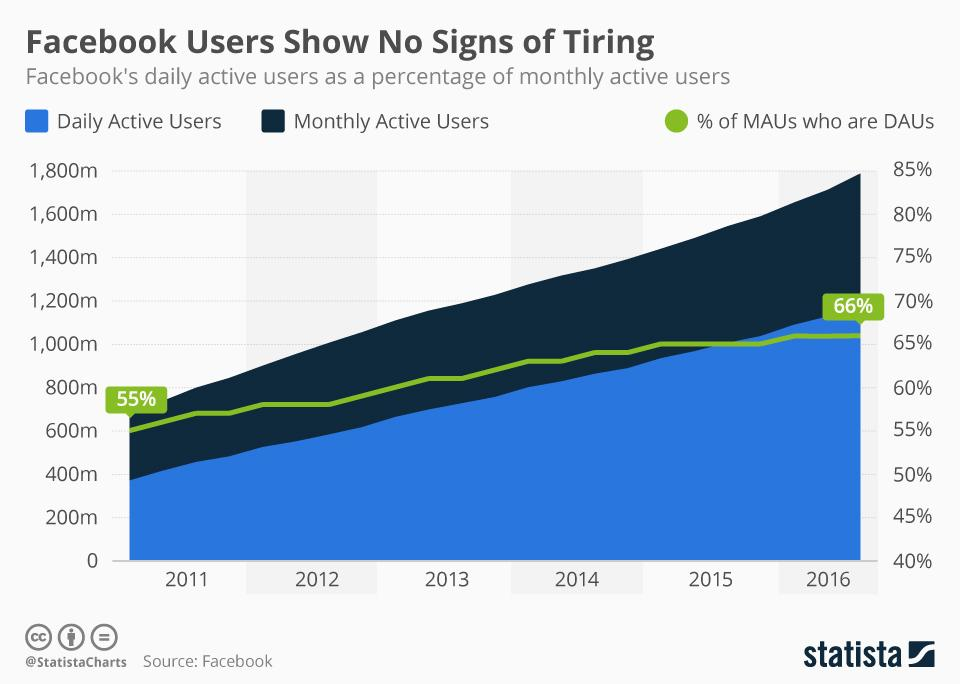
\includegraphics[width=12cm]{images/image5}
\centering
\caption[Figura 3.1]{Evolució de l’activitat diària i mensual dels usuaris de Facebook.}
\centering
\end{figure}

\subsection{Objectiu principal}

L’objectiu principal del projecte és la implementació d’una xarxa social adaptada a les persones amb diversitat funcional de dèficit cognitiu de grau mitja/baix.

\subsection{Objectius específics}

A part de l’objectiu principal del projecte, tenim uns quants objectius específics, els quals alguns d’aquest, ajuden a complir amb l’objectiu principal del projecte:

\begin{itemize}
	\item Disseny d’una interfície gràfica fàcilment manejable per persones amb baix nivell d’escriptura.
	\item Implementació d’una eina de gestió/monitoratge per a les associacions o professionals en l’àmbit.
	\item Dissenyar la xarxa social de forma que sigui responsive als diferents dispositius en els quals es podrà visitar.
	\item Implementar un sistema de seguretat, de forma que la gent que utilitzi la xarxa social siguin els usuaris amb diversitat funcional de dèficit cognitiu o professionals relacionats en l’àmbit.
	\item Implementar la xarxa de forma que accepti diferents idiomes.
\end{itemize}

\chapter{Gestió del Projecte}

\section{Abast}

L’abast del projecte vindrà donat per la implementació de dos elements essencials:

\begin{itemize}
	\item La implementació de la xarxa social per a persones amb diversitat funcional de dèficit cognitiu. Per satisfer aquest objectiu s’ha de pensar en les funcionalitats mínimes que ha de satisfer una xarxa social. Les funcionalitats mínimes que tindrà el sistema, seran les següents:
	\begin{itemize}
		\item L’usuari podrà publicar adreces d’interès, fotografies o simplement text (possiblement acompanyat d’iconografia) al seu mur.
		\item L’usuari es podrà fer amic dels altres usuaris per tal que aquests puguin veure les publicacions del seu mur.
		\item L’usuari podrà marcar “M’agrada” a les publicacions dels altres usuaris (sempre i quan siguin amics).
	\end{itemize}
	\item La implementació d’una eina de gestió per tal que els professionals de l’àmbit puguin gestionar i interactuar amb les persones que tracten en el món real. Les funcionalitats mínimes que tindrà el sistema són:
	\begin{itemize}
		\item Possibilitat d’invitar a persones amb diversitat funcional de dèficit cognitiu a entrar al sistema.
		\item Possibilitat de veure les publicacions de tots els usuaris que ha invitat.
	\end{itemize}
\end{itemize}

\subsection{Possibles obstacles}

Com en qualsevol projecte hi poden haver diversos obstacles, els quals poden dificultar el desenvolupament del software. Els obstacles possibles serien els següents:

\begin{itemize}
	\item \textbf{Temps limitat:} \\Aquest projecte té un temps bastant limitat, ja que té una data d’entrega fixa. Si no es té una bona organització del que s’ha de fer en cada moment, poden aparèixer imprevistos que puguin paralitzar el projecte. Per això, és necessari tindre una bona planificació, deixant un marge de temps per possibles imprevistos que puguin aparèixer.
	\item \textbf{Desconeixement de les tecnologies utilitzades:} \\Per desenvolupar el sistema s’utilitzaran tecnologies web i bases de dades no relacionals (Graph Database). Si aquestes no es coneixen prou, pot comportar que el desenvolupament del sistema sigui més lent i sense la qualitat suficient.
	\item \textbf{Accés a internet:} \\L’usuari del sistema necessitarà internet per poder fer-ne ús. Si aquest no té internet, aleshores no tindrà accés a la xarxa social i per tant no podrà interaccionar amb ningú mitjançant aquest sistema.
\end{itemize} 

\section{Metodología i rigor}

\subsection{Metodologies de treball} 

Per desenvolupar el projecte, s’utilitzarà scrum, el qual tractarà de definir diferents històries d’usuari (les quals representaran funcionalitats del sistema o necessitats del desenvolupador) amb uns certs punts d’història. Seguidament, es fixaran diferents dates en les quals, s’haurà d’haver acabat les històries d’usuari definides anteriorment (sempre per ordre de prioritat que el desenvolupador trobi oportú).\\ \\
Sí que és veritat que les metodologies àgils van molt encarades als treballs en grup, però considero que tot i ser un treball individual es poden aprofitar moltes idees per tal que el projecte aconsegueixi els seus objectius. Per exemple, el desenvolupament de cada funcionalitat amb completa independència de les altres.\\ \\
Les metodologies clàssiques (normalment en cascada), queden descartades, ja que el sistema que s’ha de desenvolupar tindrà moltes funcionalitats individuals, i la tecnologia en cascada, moltes vegades, implica fer canvis a les altres funcionalitats per tal d’aconseguir-ne una de nova.

\subsection{Eines de seguiment} 

En tractar-se d’un projecte software, considero que les eines de control de versions (Github i Bitbucked) són essencials. D’aquesta forma garantim que sempre tenim el codi disponible i que podem recuperar el codi anterior en cas que tinguem errors en les noves implementacions.


\subsection{Metodologies de treball} 

Per validar l’estat del projecte es passaran Unit Test, el qual tracta en testejar cadascuna de les funcionalitats del sistema un cop desenvolupades.\\ \\
A part, hi haurà vàries reunions amb el director per tal de garantir que el projecte segueix el camí establert inicialment.

\section{Planificació temporal}

\subsection{Planificació general}

\subsubsection{Durada estimada del projecte}

La durada estimada del projecte és de 6 mesos i mig, tenint en compte que el seu principi es troba en el moment en què vaig començar a fer recerca sobre el tema a tractar, principis de Desembre del 2016, i definint com a data final el dia de la defensa, que és a finals de Juny del 2017.

\subsubsection{Recursos}

Els recursos previstos per la realització d’aquest projecte són:

\begin{itemize}
	\item Recursos personals: Una persona, amb una dedicació al projecte de 25 hores setmanals.
	\item Recursos materials: Els recursos que s’utilitzaran en aquest projecte són els següents:
	\begin{itemize}
		\item \textbf{Control de versions:} Github o Bitbucked.
		\item \textbf{Servidor:} Perquè la pàgina estigui oberta les 24 hores del dia i els seus usuaris en puguin fer ús. A més, és on es trobarà la base de dades.
		\item \textbf{Correu Electrònic:} Per poder comunicar-me amb la gent que em faci falta per poder avançar el projecte.
		\item \textbf{WebStorm:} Framework de JetBrains per al desenvolupament Web.
		\item \textbf{Neo4j:} Base de dades no relacional (Graph Database), on es guardarà tota la informació dels usuaris.
		\item \textbf{GoogleDocs:} Eina d’edició de text que ens servirà per fer tota la documentació del projecte.
	\end{itemize}
\end{itemize}

\subsubsection{Pla d’acció i valoració d’alternatives}

La planificació del projecte es preveu flexible i modificable segons el ritme de desenvolupament del projecte.\\ \\
Es poden produir desviacions temporals en els diferents sprints o en el temps de dedicació a aprendre el funcionament d’una eina nova. Com que utilitzem una metodologia àgil, la qual implica crear sprints amb històries d’usuari (representen funcionalitats individuals del sistema i es mesuren en punts d’història), si una història no s’ha pogut acabar per un sprint, es ficarà pel següent. En el cas que els punts d’història que no s’han complert en un sprint siguin molt elevats, s’haurà de fer una replanificació del projecte, retallant alguna de les funcionalitats establertes a l’inici, per tal de tenir temps d’acabar-lo.\\ \\
Tot hi això, també es planificarà un sprint opcional, que ens servirà per desenvolupar funcionalitats extra en cas que les dates del projecte s’estiguin complint.

\subsubsection{Consideracions globals}

Encara que s'utilitzi una metodologia àgil, el projecte serà dut a terme per una sola persona, cosa que implica que no hi haurà desenvolupament de tasques en paral·lel. A més, es farà una llista de tasques, les quals és duran a terme seqüencialment, ordenades per prioritat del desenvolupador.\\ \\
Finalment, com que només hi haurà una persona que gestioni tot el projecte, el camí crític per satisfer totes les tasques és l’únic camí,  i per tant, trobem innecessari fer un diagrama de Pert.

\subsection{Descripció de les tasques}

\subsubsection{Posada en marxa}
En aquesta fase, l’autor farà recerca de la informació sobre el domini del projecte, necessària per al desenvolupament, i es prepararà l’entorn de treball. A més, es parlarà amb les parts interessades necessàries per resoldre els dubtes que es puguin ocasionar. Aquesta fase no té cap dependència de precedència.
	
\subsubsection{Gestió del Projecte (GEP)}
Aquesta fase consta de l’elaboració del document de gestió del projecte a partir de l’assignatura GEP. Aquesta fase no té cap dependència de precedència, però si que té un calendari estricte a seguir, ja que totes les entregues vénen donades en unes dates fixes.

\subsubsection{Desenvolupament de la xarxa social}
Elaboració de la primera part del producte, amb totes les fases del cicle de vida del desenvolupament d’un software incloses.  Aquesta tasca consistirà a desenvolupar tota la xarxa social, en la qual ja podrà ser usable pels usuaris. A més, es seguirà el següent seguit de fases: Planificació, Disseny, Implementació i Testeig. Les dependències de precedència d’aquesta etapa són les dues anteriors (Posada en marxa i Gestió del projecte).

\subsubsection{Desenvolupament de l’eina de gestió}
Elaboració de la segona part del producte, amb totes les fases del cicle de vida del desenvolupament d’un software incloses. Aquesta tasca consistirà a desenvolupar tota l’eina de gestió de la xarxa social, en la qual ja podrà ser usable pels professionals en l’àmbit. A més, es seguirà el següent seguit de fases: Planificació, Disseny, Implementació i Testeig. La dependència de precedència d’aquesta etapa és l’anterior (Desenvolupament de la xarxa social).

\subsubsection{Millores}
Opcional. Última tasca de desenvolupament del producte, on es contemplarà millores de funcionament o l’addició funcionalitats secundàries. Les dependències de precedència d’aquesta etapa són les dos anteriors (Desenvolupament de la xarxa social i Desenvolupament de l’eina de gestió).

\subsubsection{Documentació i Defensa}
Aquesta fase consistirà a acabar tota la documentació (memòria del projecte) i revisar que aquesta sigui correcta. La documentació s’anirà fent en les fases anteriors. A part, també es prepararà la defensa del projecte.\\ \\
La memòria del projecte inclourà tota la documentació redactada en el mòdul de GEP i la documentació derivada de les fases anteriors. El document final i la defensa tenen com a precedència totes les tasques anteriors del projecte.
\newpage
\subsection{Calendari}

\subsubsection{Estimació d'hores}

\begin{table}[h]
\centering
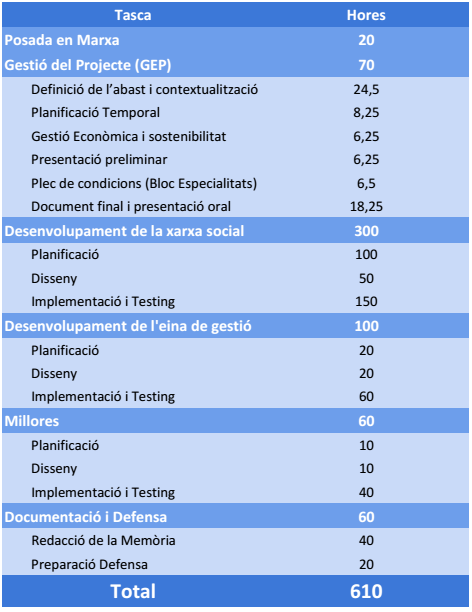
\includegraphics[width=12cm]{images/taula1}
\caption[Taula 6.1]{Estimació d'hores}
\centering
\end{table}

\newpage

\subsubsection{Diagrama de Gantt}

\begin{figure}[h]
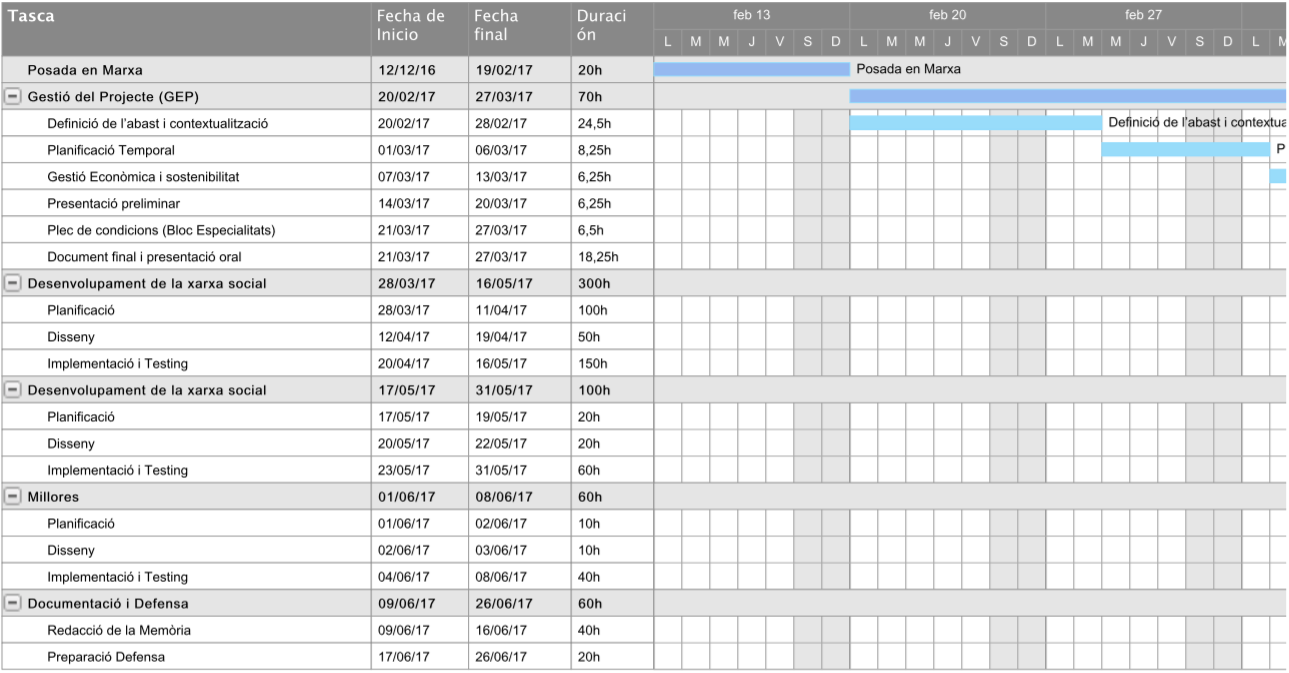
\includegraphics[width=12cm]{images/image2}
\centering
\end{figure}

\begin{figure}[h]
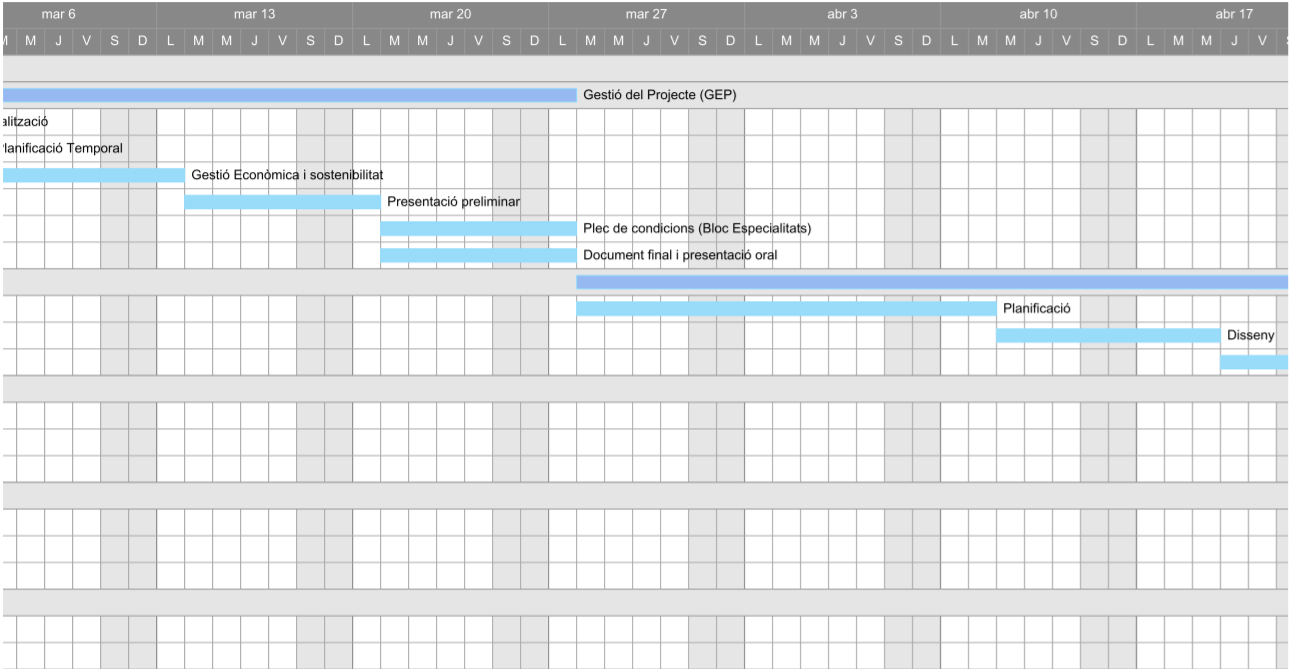
\includegraphics[width=12cm]{images/image8}
\centering
\end{figure}

\begin{figure}[h]
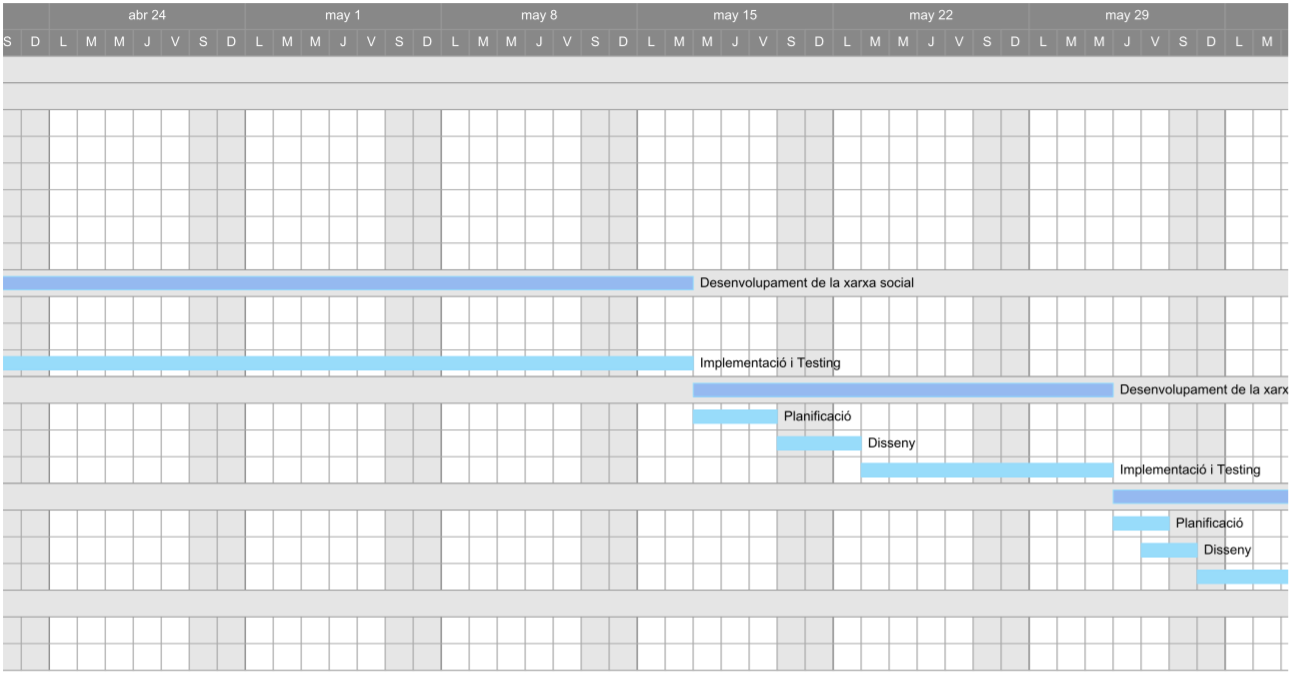
\includegraphics[width=12cm]{images/image4}
\centering
\end{figure}

\begin{figure}[h]
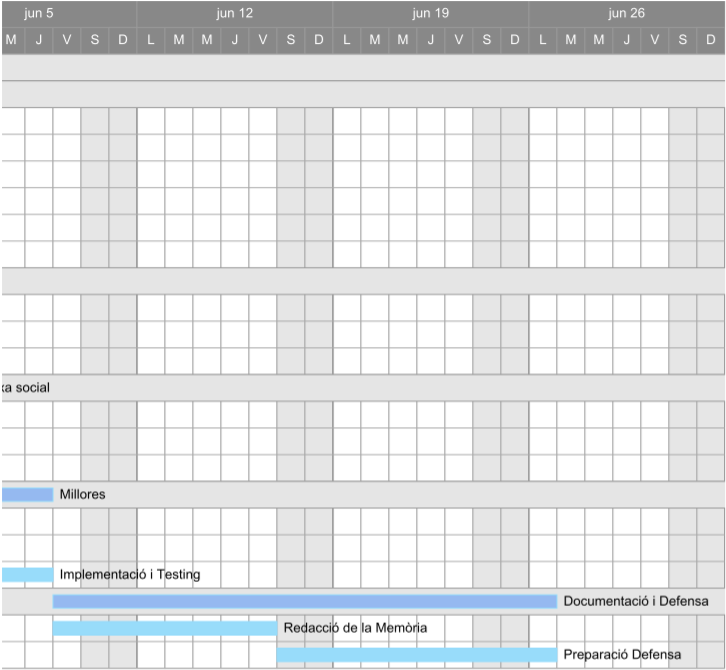
\includegraphics[width=12cm]{images/image7}
\centering
\caption[Figura 6.1]{Diagrama de Gantt}
\centering
\end{figure}

\section{Gestió Econòmica}

\subsection{Consideracions inicials}

En aquesta secció, identificarem tots els recursos necessaris per a la realització del projecte i farem una estimació del cost total d’aquests, tenint en compte aquestes dues variants:
\begin{itemize}
	\item Assumim que el projecte és universitari, i que per tant, no té una inversió econòmica.
	\item Assumim que és un projecte competitiu, amb les hores de recursos humans a preu de mercat.
\end{itemize}
A més, també s’explicarà com es durà a terme el control de la gestió durant tot el projecte.

\subsection{Identificació i estimació de costos}

\subsubsection{Costos directes}

Els costos directes per activitat en aquest projecte inclouen els recursos humans involucrats en cada una de les activitats definides al diagrama de Gantt presentat anteriorment. Encara que a la pràctica tot el projecte estigui desenvolupat per una sola persona, cada activitat d’aquest correspon a un rol diferent, i per tant, les hores tindran un preu de mercat diferent:

\begin{itemize}
	\item Tasques de gestió i documentació (Cap de Projecte): 50€/h.
	\item Anàlisis i disseny del producte (Analista): 40€/h.
	\item Implementació i proves (Programador): 35€/h.
\end{itemize}

A continuació trobem una taula amb el cost de mercat i el cost estimat d’aquest projecte:

\begin{table}[H]
\centering
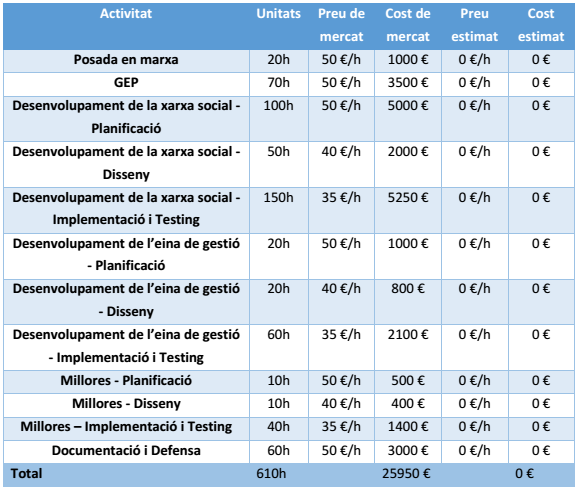
\includegraphics[width=15cm]{images/taula2}
\caption[Taula 7.1]{Costos directes}
\centering
\end{table}

\subsubsection{Costos indirectes}

En aquesta secció tindrem en compte tots els costos que ens afectin de forma indirecta, ho sigui, considerarem tots els costos que siguin necessaris pel projecte que siguin necessàries per a qualsevol projecte de software o que s’hagin de considerar en aquest projecte.
\begin{itemize}
	\item \textbf{Transport:} S’utilitzarà un abonament trimestral de 105 €. Com que l’abonament no depèn del nombre de viatges, considerarem que el cost extra és de 0%.
	\item \textbf{Software Extern:} S’intentarà fer servir software lliure i gratuït, de forma que el seu cost serà 0.
	\item \textbf{Impressions de paper:} el lliurament del projecte, inclou el lliurament de documentació. Suposarem que l’extensió de la memòria és d’unes 150 pàgines. Per altra banda, se’n han de fer 4 copies: 3 per als membres del tribunal i una pel director del projecte. Comptarem que cada pàgina costa uns 0,05 € (enquadernació inclosa).
	\item \textbf{Hardware:} L’únic hardware que s’utilitzarà en aquest projecte és un ordinador portàtil que ja es troba en ús. Suposant que la vida útil d’un portàtil és de 5 anys i que el 60\% del seu ús durant els propers 4 mesos estarà dedicat al projecte.
	\item \textbf{Connexió a internet:} Tot i que la connexió a internet és imprescindible per quasi qualsevol informàtic, considerarem que ja existeix una contractació. A partir d’aquí suposarem que de l’ample de banda consumit, se’n dedica un 20\% al projecte durant el temps que aquest duri.
\end{itemize} 

\begin{table}[h]
\centering
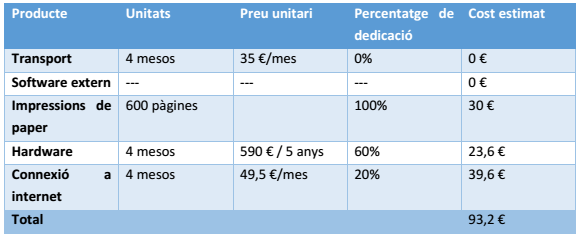
\includegraphics[width=15cm]{images/taula3}
\caption[Taula 7.2]{Costos indirectes}
\centering
\end{table}

\subsubsection{Contingència}

Per evitar qualsevol rics que hi pugui haver, reservarem una part del pressupost per a la part de contingència. Aquest cost serà un 15\% de la suma dels costos directes i indirecte.

\begin{table}[h]
\centering
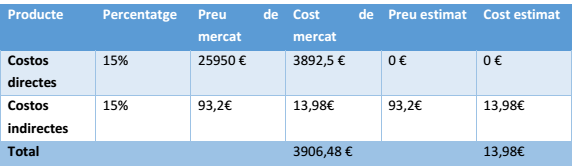
\includegraphics[width=15cm]{images/taula4}
\caption[Taula 7.3]{Contingència}
\centering
\end{table}

\subsubsection{Imprevistos}

Durant el projecte es poden presentar diferents imprevistos que ens facin encarir el projecte, els quals són:
\begin{itemize}
	\item \textbf{Avaria ordinador:} en cas que hi hagués algun problema amb el hardware, s’hauria de reparar o comprar-ne un de nou, augmentant el cost del projecte en màxim el preu de l’ordinador nou. Assignarem a aquesta eventualitat una probabilitat del 5\%.
	\item \textbf{Retard de 8 dies:} com que en la planificació temporal ja hem fet una reserva de millores del projecte, en cas de que aquest s’allargui s’utilitzarà aquesta reserva per acabar-lo.
\end{itemize}

\begin{table}[H]
\centering
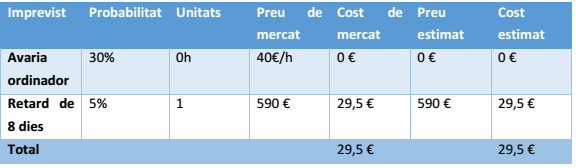
\includegraphics[width=15cm]{images/taula5}
\caption[Taula 7.4]{Imprevistos}
\centering
\end{table}

\subsubsection{Pressupost}

Durant el projecte no es consideren les següents situacions:
\begin{itemize}
	\item No es tenen en compte els augments de preu (escalació) durant el projecte, ja que es de curta durada i no es preveu que es doni la situació.
	\item No hi ha cap marge de benefici, ja que el projecte és completament sense ànim de lucre i no està destinat a la venda d’un producte.
\end{itemize}

\begin{table}[H]
\centering
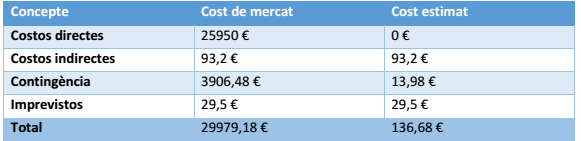
\includegraphics[width=15cm]{images/taula6}
\caption[Taula 7.5]{Pressupost}
\centering
\end{table}

\subsection{Control de gestió}

Per poder preveure les desviacions a nivell de temps, durant la realització del projecte, es mantindrà un registre d’hores amb data i concepte per tal de veure si es sobrepassa el número d’hores planificat. A més, a l’hora de fer cada una de les iteracions, com ja hem especificat a l’apartat de metodologia i rigor, és durà a terme amb metodologies àgils, cosa que ens donarà bastant marge de planificació en el cas que preveiem que s’hagi d’allargar el projecte, ja que les metodologies àgils ens donen l’opció de fragmentar molt les tasques en tasques més petites.\\ \\
Al final del projecte, quan ja es tinguin les hores reals que s’han dedicat al projecte i els costos indirectes, es farà una comparació amb la previsió inicial.\\ \\
En cas de que la comparativa sigui molt extrema es mirarà quines han sigut les causes que han provocat aquesta situació. Si el cost real ha sigut major al pressupostat, es mirarà si ha sigut degut als imprevistos que s’han tingut en compte i si es pot cobrir amb la partida corresponent. Si no es pot, s’assignarà la partida de contingència per cobrir-ho. Només es tindran en compte els costos indirectes, la partida d’imprevistos i la partida de contingència.

\section{Sostenibilitat i compromís social}

En aquest apartat, es farà una breu descripció de com afecta el projecte a nivell econòmic, social i ambiental.

\begin{table}[H]
\centering
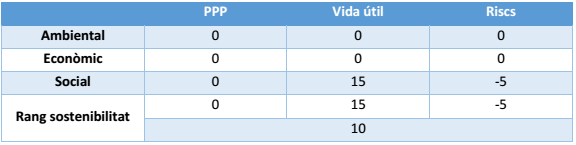
\includegraphics[width=15cm]{images/taula7}
\caption[Taula 7.5]{Pressupost}
\centering
\end{table}

\subsection{Econòmica}

Com que el projecte és sense ànim de lucre, he decidit punta’l en 0 punts a nivell econòmic. Ja que no està pensat per fer-hi negoci, sinó a ser una eina que ajudi a integrar a la societat totes aquelles persones que ho necessiten i no tenen l’oportunitat de fer-ho.

\subsection{Social}

L’objectiu principal del projecte, és donar l’opció de poder utilitzar una xarxa social a persones amb diversitat funcional de dèficit cognitiu amb unes nocions mínimes de lectura i escriptura. Per tant, com que el projecte està encarat a fer una ajuda social, he decidit ficar-li 15 punts d’impacte social. \\ \\
També existeix algun risc social en aquest projecte, ja que pot haver-hi persones que el categoritzin de marginació social pel fet de que només i tinguin accés persones amb diversitat funcional de dèficit cognitiu, o professionals relacionats en l’àmbit. Per això, he decidit ficar-li -5 punts de risc social.

\subsection{Ambiental}

He decidit puntuar tota la secció ambiental amb 0 punts, ja que el projecte no ajuda ni perjudica el medi ambient. A més no és preveu la dependència de cap recurs en acabar el projecte, ni necessitarem cap producte nou.


\chapter{Seguiment del Projecte}

\section{Introducció}

En aquest capítol, es definirà quin ha sigut el seguiment del projecte i com s'ha dut a terme. \\ \\
Ja que en el projecte s'utilitzen les metodologies àgils, s'ha definit un product backlog inicial amb totes les històries a realitzar durant el projecte. A més, la planificació temporal s'ha dividit en 6 sprints:
\begin{itemize}
	\item 3 Sprints pertinents al desenvolupament de la xarxa social.
	\item 2 Sprints pertinents al desenvolupament de l'eina de gestió.
	\item 1 Sprint pertinant a la part de millores.
\end{itemize}
Abans de realitzar cada un dels sprints, es seleccionen les històries del backlog que es realitzaràn. Quan aquest finalitza, les històries que no s'han acabat es retornen al backlog, o en casos molt específics, es descarten del projecte.\\ \\
En aquesta secció es descriurà quin ha sigut el backlog inicial, i com s'ha procedit en cada un dels sprints.
\newpage
\section{Product Backlog}

El product backlog inicial del projecte ha sigut el següent:

\begin{table}[H]
\centering
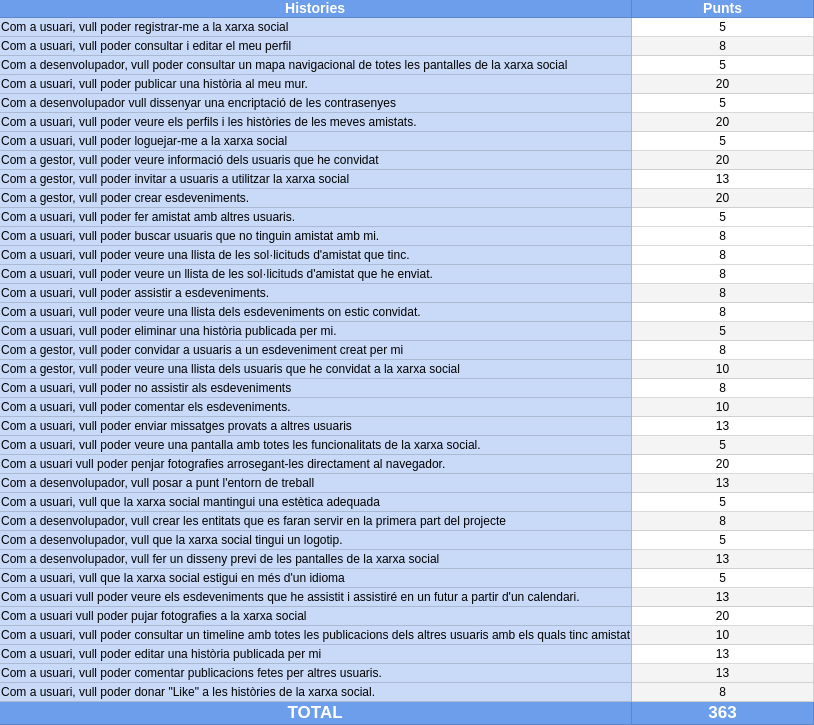
\includegraphics[width=15cm]{images/taula8}
\caption[Taula 7.5]{Product Backlog}
\centering
\end{table}

\section{Sprint 1}

\subsection{Resum de l'sprint}

L’sprint no ha anat dins dels marges esperats. Dels 64 punts definits en aquest sprint, només se’n han aconseguit 31.\\ \\
Això es deu al poc coneixement de les tecnologies que s’havien d’utilitzar a priori, i que per tant s’ha fet molt difícil a l’hora d’utilitzar-les. També cal dir que moltes d’aquestes tecnologies s’han hagut de buscar en el moment que ha sortit la necessitat d’utilitzar-les i s’han convertit en requisits emergents dins del projecte.\\ \\
En els apartats següents veurem quines són les tasques que s’han dut a terme en aquest sprint i quin ha sigut el seu resultat. 

\subsection{Descripció i resultat de les històries d’usuari}

\subsubsection{Com a desenvolupador, vull posar a punt l'entorn de treball (13 punts)}

Aquesta història a consistit en buscar i instal·lar totes les tecnologies necessàries per posar en marxa el projecte. S’ha dividit en les següents tasques:
\begin{itemize}
	\item Instal·lar IntellIJ Webstorm.
	\item Instal·lar Node.js.
	\item Buscar servei de núvol on puguem penjar la pàgina web.
	\item Instal·lar els paquets necessaris de Node.js.
	\item Creació del repositori de GitHub.
\end{itemize}
\textcolor{forestgreen}{\textbf{Resultat:}} Totes les tasques que s’han descrit en aquesta història s’han completat en el temps estimat. El problema ha vingut a l’hora de començar ha implementar la història "Com a usuari, vull poder registrar-me a la xarxa social" de l’sprint (la qual veurem més endavant), ja que hi ha hagut molts requisits emergents que no s’han tingut en compte anteriorment, i per tant, el temps d’aquesta història a augmentat moltíssim.

\subsubsection{Com a usuari, vull que la xarxa social mantingui una estètica adequada (5 punts)}

Aquesta història  ha consistit en buscar els colors o fonts (tipus de lletra) per a que la pàgina web tingui una estètica agradable a la vista de l’usuari. S’ha dividit en les següents tasques:
\begin{itemize}
	\item Buscar els colors primaris.
	\item Buscar una font.
\end{itemize}
\textcolor{forestgreen}{\textbf{Resultat:}} No ha sigut molt difícil trobar els colors primaris i les fonts principals de l’aplicació. Els colors primaris són els següents:

\begin{figure}[h]

\includegraphics[width=12cm]{images/image1}
\centering
\caption[]{Paleta de colors de l'aplicació.}
\centering
\end{figure}

Per troba’ls, he utilitzat un eina que es diu \textbf{paletton}, la qual et permet combinar colors de forma senzilla. Per utilitzar-la podeu entrar a la següent URL: \\ \\
\url{http://paletton.com/\#uid=5300u0kqALsd8VjkyQ8B3GbBuoR} \\ \\
L’aplicació estarà composta per dos fonts:
\begin{itemize}
	\item \textbf{Montserrat:} És la font que s’utilitzarà en els títols.
	\item \textbf{Raleway:} S’utilitzarà per la resta de text de l’aplicació.
\end{itemize}

\subsubsection{Com a desenvolupador, vull crear les entitats que es faran servir en la primera part del projecte (8 punts)}

Aquesta història ha consistit en crear les entitats de dades que guardarem a la base de dades. S’ha dividit en les següents tasques:
\begin{itemize}
	\item Creació de l’entitat “Usuari”
	\item Creació de l’entitat “Història”
	\item Creació de l’entitat “Esdeveniment”
\end{itemize}
\textcolor{forestgreen}{\textbf{Resultat:}} Aquesta història va tenir una molt mala estimació de cost, ja que el temps en que s’ha realitzat ha sigut bastant ràpid. Les entitats resultants són les següents:

\begin{figure}[h]
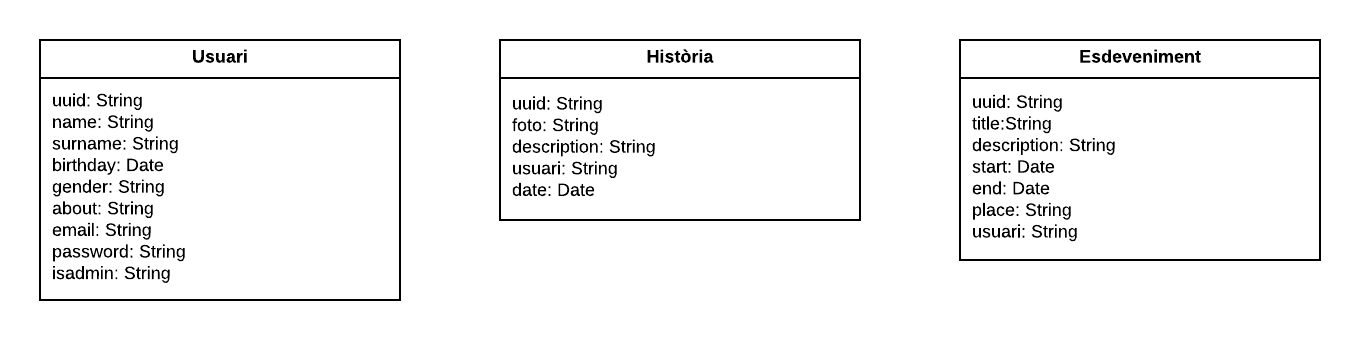
\includegraphics[width=15cm]{images/image6}
\centering
\caption[]{Entitats de l'aplicació.}
\centering
\end{figure}

\subsubsection{Com a desenvolupador, vull que la xarxa social tingui un logotip (5 punts)}

Aquesta història ha consistit en la creació d’un logotip per utilitzar en la nostra aplicació web. S’ha dividit en les següents tasques:
\begin{itemize}
	\item Buscar Imatges pel logotip.
	\item Creació del logotip.
\end{itemize}
\textcolor{forestgreen}{\textbf{Resultat:}} La tasca s’ha realitzat correctament, i dins de l’estimació donada en punts. Per fer el logotip de l’aplicació, s’han utilitzat les mateixes fonts que s’han triat en la història "Com a usuari, vull que la xarxa social mantingui una estètica adequada" d’aquest sprint. 
El resultat és el següent:

\begin{figure}[H]

\includegraphics[width=7cm]{images/image3}
\centering
\caption[]{Logotip de l'aplicació.}
\centering
\end{figure}

\subsubsection{Com a desenvolupador, vull poder consultar un mapa navegacional de totes les pantalles de la xarxa social (5 punts)}

\textcolor{costumyellow}{\textbf{Resultat:}} Com hem vist anteriorment, la història "Com a desenvolupador, vull posar a punt l'entorn de treball" d’aquest sprint ens a fet perdre molt temps. Temps que s’hagués pogut invertir en fer la resta d’històries. Per tant, al veure que no necessitàvem un mapa navegacional en aquest  sprint, he decidit deixar aquesta història per l’sprint 2.

\subsubsection{Com a desenvolupador, vull fer un disseny previ de les pantalles de la xarxa social (13 punts)}

\textcolor{red}{\textbf{Resultat:}} Durant l’sprint, a l’hora de ficar-me a fer aquesta història, em vaig adonar que el cost d’aquesta era molt elevat, i que per tant era una pèrdua de temps fer aquest disseny. Comptant que el temps per fer el projecte és molt poc i que el seu valor no és molt elevat pel projecte, he decidit retirar aquesta història.

\subsubsection{Com a usuari, vull que la xarxa social estigui en més d'un idioma (5 punts)}

\textcolor{red}{\textbf{Resultat:}} Vaig estar buscant alguna forma de simplificar l’aplicació i ficar els literals (paraules fixes que es troben a l’aplicació) en un mateix fitxer. La solució que vaig trobar era bastant difícil d’implementar i feia pujar els punts d’aquesta història. Conseqüentment, he optat que per cada pàgina de l’aplicació, hi haurà 3 versions (una en anglès, una en castellà i una altra en català). Per tant, la història es retira del backlog inicial.

\subsubsection{Com a usuari, vull poder registrar-me a la xarxa social (5 punts)}

\textcolor{costumyellow}{\textbf{Resultat:}} La història "Com a desenvolupador, vull posar a punt l'entorn de treball" ens ha tret molt de temps d’aquest sprint, i conseqüentment, aquesta història no s’ha pogut acabar i queda per l’sprint 2.

\subsubsection{Com a usuari, vull poder loguejar-me a la xarxa social (5 punts)}

\textcolor{costumyellow}{\textbf{Resultat:}} La història "Com a desenvolupador, vull posar a punt l'entorn de treball" ens ha tret molt de temps d’aquest sprint, i conseqüentment, aquesta història no s’ha pogut ni començar i queda per l’sprint 2.

\subsection{Tecnologies utilitzades}

\subsubsection{Tecnologies Web}

Aquesta tecnologia és necessària per al funcionament de l’aplicació. Si l’aplicació no es troba en al núvol, aquesta no és accessible pels usuaris, i per tant perd el seu valor. \\ \\
La tecnologia que he triat per utilitzar és diu Heroku (\url{https://www.heroku.com}), i és una plataforma d’aplicacions al núvol. Aquesta plataforma permet tindre la teva pàgina web online les 24h, i a més, té un sistema de storage, on es guarden totes les dades generades pels usuaris de la pàgina.\\ \\
La URL a la pàgina on es troba l’aplicació d’aquest projecte és: \\
\url{https://makeyourfriend.herokuapp.com}

\subsubsection{IDE}

Com que el projecte és web, també s’ha d’utilitzar una IDE encarada ha aquest propòsit. La que he triat per aquest projecte es diu IntellIJ WebStorm (\url{https://www.jetbrains.com/webstorm}), i és una IDE que està encarada al Javascript, però que també accepta tot el que vindria a ser els llenguatges de frontend, com HTML o CSS.\\ \\
La llicencia d’aquesta IDE, és de pagament, però al ser estudiant de la FIB et surt gratuïta.

\subsubsection{Bases de Dades}

Com que l’aplicació és una xarxa social, una base de dades relacional no és tant eficient, ja que sempre ha d’estar buscant a les taules. Conseqüentment, he decidit utilitzar una base de dades no relacional anomenada neo4j (\url{https://neo4j.com}). Aquesta base de dades és una graph database que permet crear nodes (on es guarda la informació de l’usuari, històries o esdeveniments) i seguidament relacionar-los entre ells amb una etiqueta. \\ \\
La seva eficiència en aquest tipus d’aplicacions, cau en que no cal que tinguem una taula amb totes les amistats. Si volem saber quines amistats té un usuari, ens fiquem al node d’aquest usuari i mirem les arestes que contenen el tag “Amistat”. Aquestes arestes ens porten directament als nodes de les amistats.\\ \\
Finalment, ni que en aquest sprint no s’hagi fet, segurament serà necessari una base de dades relacional per emmagatzemar les fotografies de l’aplicació i guanyar eficiència. Quan una fotografia es guarda en una base de dades, s’encripta amb un string (que ocupa molt espai), i per tant, costaria molt fer una cerca per la base de dades.

\subsubsection{Framework}

El framework utilitzat pel projecte és Node.js (\url{https://nodejs.org}). És un framework que et facilita totes les feines encarades a web. Els seus llenguatges bàsics són HTML, CSS i Javascript, tot i que pots afegir les funcionalitat que vulguis instal·lant els paquets necessaris al teu projecte.\\ \\
Finalment, dir que aquest framework et dona molta facilitat per implementar la comunicació client servidor.

\subsubsection{Paquets addicionals de Node.js}

Com he dit a l’apartat anterior, Node.js et permet instal·lar paquets amb funcionalitats extra al teu projecte. Els paquets que s’ha utilitzat en aquest sprints són els següents:
\begin{itemize}
	\item \textbf{body-parser:} Aquest paquet ens permet llegir els camps que ha omplert el client directament des del servidor, sense la necessitat d’haver de fer una crida ajax per passar els paràmetres.
	\item \textbf{bootstrap:} És un framework per HTML, CSS i Javascript que permet fer les pàgines responsive amb facilitat.
	\item \textbf{dotenv:} ens permet carregar fitxers .env a l’aplicació.
	\item \textbf{jquery:} És una llibreria de Javascript que et permet escriure el mateix codi de forma més ràpida, i que permet la manipulació del codi HTML de forma senzilla.
	\item \textbf{jquery-validation:} És un pluguin de jQuery que serveix per validar els diferents formularis que hi puguin haver a l’aplicació (dates, correus electrònics, contrasenyes, etc).
	\item \textbf{neo4j-driver:} És un driver que permet configurar connexions amb Neo4j, ja explicat a l’apartat 3.3.
uuid: Ens permet auto generar un identificador únic per a cada node de la base de dades.
	\item \textbf{pug:} Aquest paquet permet escriure el codi HTML més ràpidament i permet crear bucles d’informació dinàmica a la pàgina web.
	\item \textbf{font-awesome:} És una llibreria d’icones.
	\item \textbf{w3-css:} Permet fer dissenys més amistosos per l’usuari de l’aplicació amb facilitat.

\end{itemize}

\subsubsection{Conclusions de l'sprint}

Com podem veure, durant aquest sprint s’han fet menys de la meitat dels punts que estaven previstos. Tot hi això, ja tenim quasi totes les tecnologies necessàries instal·lades a l’aplicació i per tant, serà més fàcil utilitzar-les.\\ \\
Si que és possible que durant l’sprint 2 sorgeixi la necessitat d’alguna tecnologia més, per preveig que seran molt poques.


\section{Sprint 2}

\section{Sprint 3}

\section{Sprint 4}

\section{Sprint 5}

\section{Sprint 6}

%%%%%%%%%%%%%%%%%%%%%%%%%%%%%%%%%%%%%%%%%%%%%%%%%%%%%%%%%%%%%%%%%%%%%%%%%%%%%%%
%                                 CONCLUSIONS                                 %
%%%%%%%%%%%%%%%%%%%%%%%%%%%%%%%%%%%%%%%%%%%%%%%%%%%%%%%%%%%%%%%%%%%%%%%%%%%%%%%

\chapter{Conclusions}

????? ????????????? ????????????? ????????????? ????????????? ????????????? 

%%%%%%%%%%%%%%%%%%%%%%%%%%%%%%%%%%%%%%%%%%%%%%%%%%%%%%%%%%%%%%%%%%%%%%%%%%%%%%%
%                                BIBLIOGRAFIA                                 %
%%%%%%%%%%%%%%%%%%%%%%%%%%%%%%%%%%%%%%%%%%%%%%%%%%%%%%%%%%%%%%%%%%%%%%%%%%%%%%%

\begin{thebibliography}{10}
%%%%%%%%%%%%%%%%%%%%%%%%%%%%%%%%%%%%%%%%%%%%%%%%%%%%%%%%%%%%%%%%%%%%%%%%%%%%%%%
% MODEL D'ARTICLE                                                             %
%%%%%%%%%%%%%%%%%%%%%%%%%%%%%%%%%%%%%%%%%%%%%%%%%%%%%%%%%%%%%%%%%%%%%%%%%%%%%%%
\bibitem{light}
   Jennifer~S. Light.
   \newblock When computers were women.
   \newblock \textit{Technology and Culture}, 40:3:455--483, juliol, 1999.

%%%%%%%%%%%%%%%%%%%%%%%%%%%%%%%%%%%%%%%%%%%%%%%%%%%%%%%%%%%%%%%%%%%%%%%%%%%%%%%
% MODEL DE LLIBRE                                                             %
%%%%%%%%%%%%%%%%%%%%%%%%%%%%%%%%%%%%%%%%%%%%%%%%%%%%%%%%%%%%%%%%%%%%%%%%%%%%%%%
\bibitem{ifrah}
   Georges Ifrah.
   \newblock \textit{Historia universal de las cifras}.
   \newblock Espasa Calpe, S.A., Madrid, sisena edició, 2008.

%%%%%%%%%%%%%%%%%%%%%%%%%%%%%%%%%%%%%%%%%%%%%%%%%%%%%%%%%%%%%%%%%%%%%%%%%%%%%%%
% MODEL D'URL                                                                 %
%%%%%%%%%%%%%%%%%%%%%%%%%%%%%%%%%%%%%%%%%%%%%%%%%%%%%%%%%%%%%%%%%%%%%%%%%%%%%%%
\bibitem{WAR}
   Comunicat de premsa del Departament de la Guerra, 
   emés el 16 de febrer de 1946. 
   \newblock Consultat a 
   \url{http://americanhistory.si.edu/comphist/pr1.pdf}.

\end{thebibliography}
\cleardoublepage

%%%%%%%%%%%%%%%%%%%%%%%%%%%%%%%%%%%%%%%%%%%%%%%%%%%%%%%%%%%%%%%%%%%%%%%%%%%%%%%
%                           APÈNDIXS  (Si n'hi ha!)                           %
%%%%%%%%%%%%%%%%%%%%%%%%%%%%%%%%%%%%%%%%%%%%%%%%%%%%%%%%%%%%%%%%%%%%%%%%%%%%%%%

\APPENDIX

%%%%%%%%%%%%%%%%%%%%%%%%%%%%%%%%%%%%%%%%%%%%%%%%%%%%%%%%%%%%%%%%%%%%%%%%%%%%%%%
%                         LA CONFIGURACIO DEL SISTEMA                         %
%%%%%%%%%%%%%%%%%%%%%%%%%%%%%%%%%%%%%%%%%%%%%%%%%%%%%%%%%%%%%%%%%%%%%%%%%%%%%%%

\chapter{Configuració del sistema}

????? ????????????? ????????????? ????????????? ????????????? ?????????????

\section{Fase d'inicialització}

????? ????????????? ????????????? ????????????? ????????????? ?????????????

\section{Identificació de dispositius}

????? ????????????? ????????????? ????????????? ????????????? ?????????????

%%%%%%%%%%%%%%%%%%%%%%%%%%%%%%%%%%%%%%%%%%%%%%%%%%%%%%%%%%%%%%%%%%%%%%%%%%%%%%%
%                               ALTRES  APÈNDIXS                              %
%%%%%%%%%%%%%%%%%%%%%%%%%%%%%%%%%%%%%%%%%%%%%%%%%%%%%%%%%%%%%%%%%%%%%%%%%%%%%%%


\chapter{??? ???????????? ????}

????? ????????????? ????????????? ????????????? ????????????? ????????????? 



%%%%%%%%%%%%%%%%%%%%%%%%%%%%%%%%%%%%%%%%%%%%%%%%%%%%%%%%%%%%%%%%%%%%%%%%%%%%%%%
%                              FI DEL DOCUMENT                                %
%%%%%%%%%%%%%%%%%%%%%%%%%%%%%%%%%%%%%%%%%%%%%%%%%%%%%%%%%%%%%%%%%%%%%%%%%%%%%%%

\end{document}
